\section{Case Study and Experiments} \label{sec:casestudy}
In this section, we will study the use of the proposed on-accelerator training framework 
on three typical scenarios including CNN accelerator with approximate multiplier, 
CNN accelerator with extreme overclocking and CNN accelerator with soft errors, 
in which the CNN accelerator produces undetermined computing result of neural networks.
Each application scenario is used as a case study and presented with comprehensive 
experiments. 

The scenarios of approximate computing and overclocking rely on the 8-bit 
fixed-point PipeCNN \cite{pipecnn_2} implemented on Xilinx KCU1500 board, 
while soft error scenario is analyzed based on an equivalent C model of PipeCNN.  
In addition, we use four representative convolution neural networks including LeNet, 
AlexNet, VGG-16 and VGG-19 as the benchmark for all the experiments. The neural networks 
are summarized in Table \ref{tab:CNN-table}. The benchmark has diverse network sizes and 
covers the typical neural network layers. Thus, the analysis can be applied to more 
neural networks.

\begin{table}
        \centering
        \vspace{-0.3em}
        \caption{Four popular CNN information}
        \label{tab:CNN-table}
        \vspace{-0.3em}
        \begin{tabular}{c|c|c|c}
		\toprule
		  & Dataset & Layers & Total weights \\
		\midrule
		LeNet & Mnist & 4 & 60K \\
		\midrule
		AlexNet & ImageNet & 8 & 61M \\
		\midrule
		VGG-16 & ImageNet & 16 & 138M \\
		\midrule
		VGG-19 & ImageNet & 19 & 143M \\
		\bottomrule
        \end{tabular}
        \vspace{-1em}
\end{table}


\subsection{CNN accelerator with approximate arithmetic logic}
Approximate arithmetic logic that promises high-performance 
and energy-efficient computing has been demonstrated to be 
beneficial to CNN accelerators and studied intensively 
in prior work. When the approximate arithmetic logic 
is used in a CNN accelerator, the computing result of a 
neural network will be different from the exact computing result.
This may further lead to prediction accuracy loss when deploying 
the neural network model directly as demonstrated in 
Section \ref{sec:motivation}. This scenario fits well with the on-accelerator 
training framework and is analyzed in this section.

We choose the dynamic-range approximate multiplier proposed in \cite{Approximate_Multiplier_31} as 
an approximate computing example and employ the multiplier on the PipeCNN
accelerator. The approximate multiplier basically reserve the most 
significant non-zero bits as well as the following $k$ lower bits. 

\begin{figure}
        \center
        \subfloat[top1]{
                \label{fig:appro-k2-top1}
                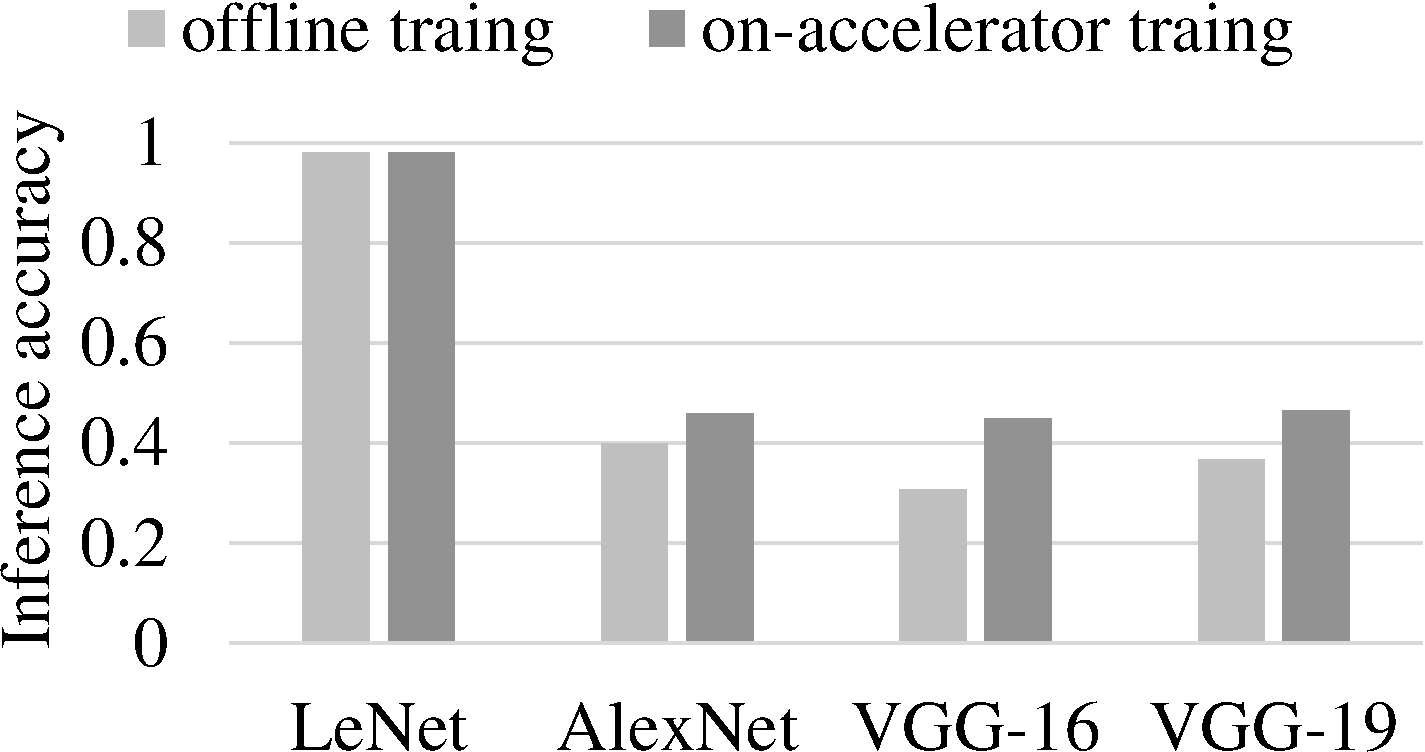
\includegraphics[width=0.6\linewidth]{appro-k2-top1}
        }
        \qquad
        \subfloat[top5]{
                \label{fig:appro-k2-top5}
                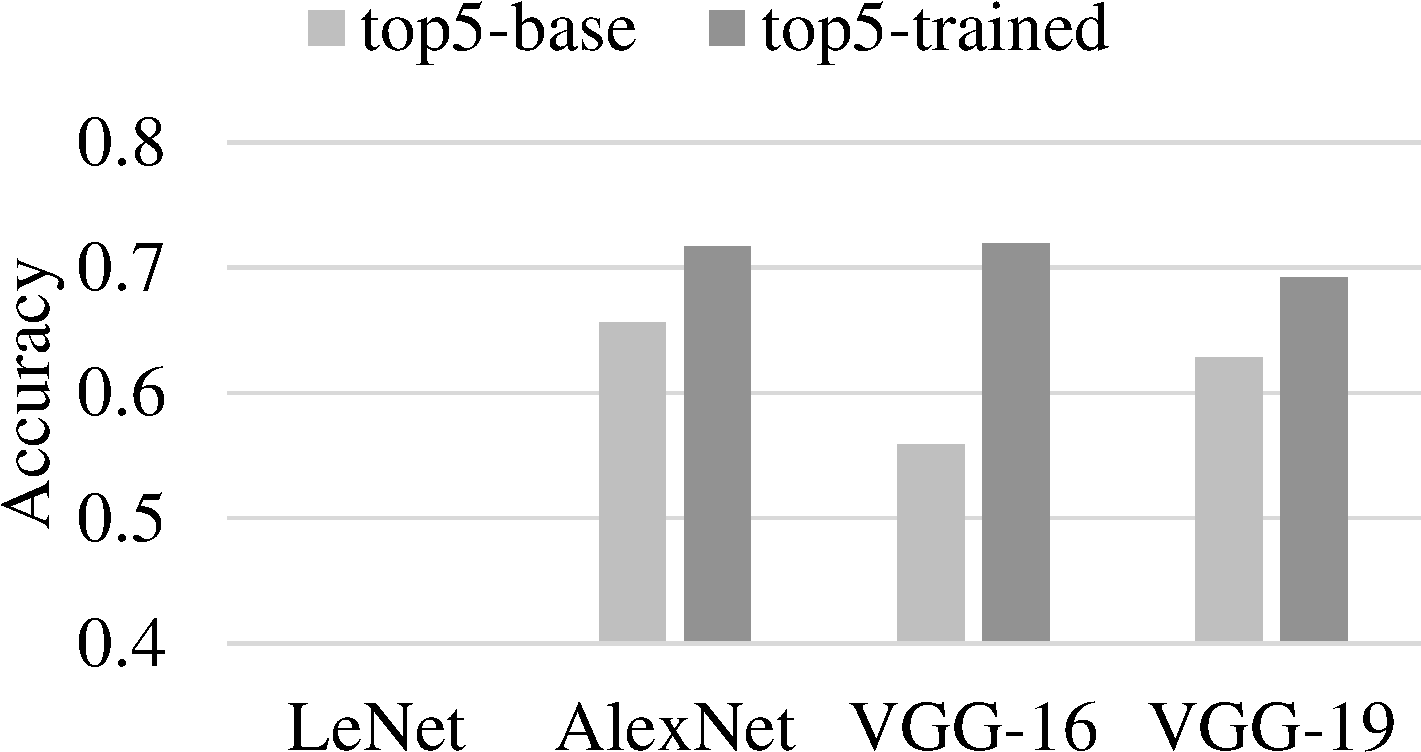
\includegraphics[width=0.6\linewidth]{appro-k2-top5}
        }
        \caption{The Accuracy of Four CNN models on accelerators with approximate multiplier(k=2)}
        \label{fig:approximate mltiplier}
\end{figure}

\begin{figure}
        \center
        \subfloat[top1]{
                \label{fig:appro-k3-top1}
                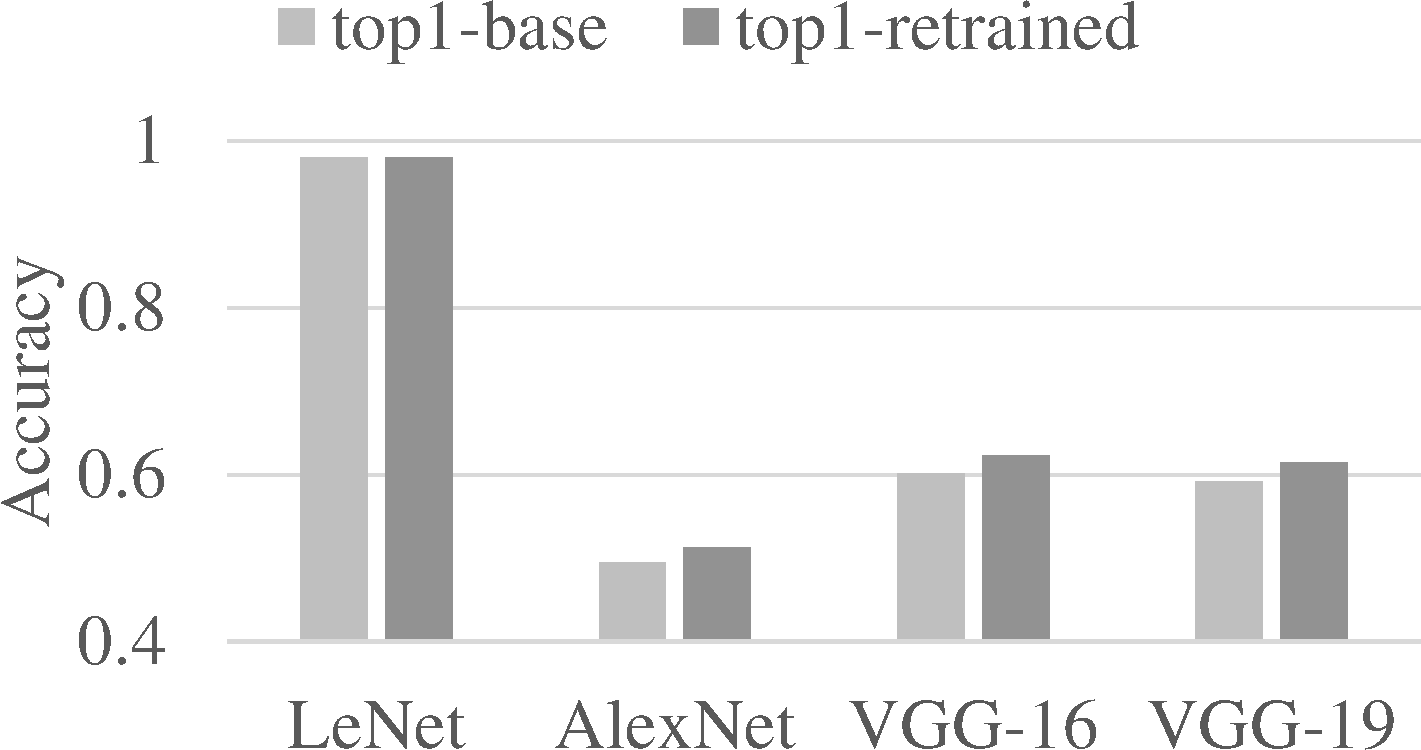
\includegraphics[width=0.6\linewidth]{appro-k3-top1}
        }
        \qquad
        \subfloat[top5]{
                \label{fig:appro-k3-top5}
                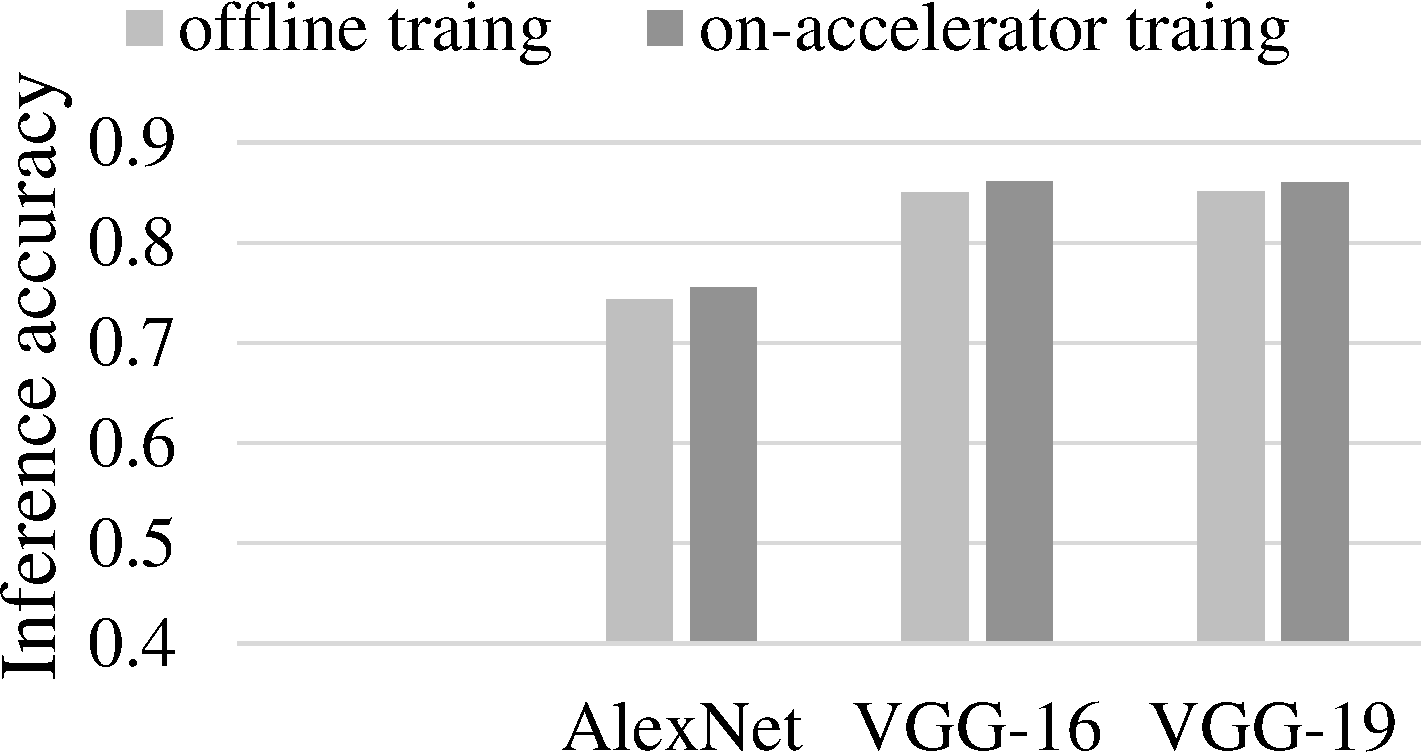
\includegraphics[width=0.6\linewidth]{appro-k3-top5}
        }
        \caption{The Accuracy of Four CNN models on accelerators with approximate multiplier(k=3)}
        \label{fig:approximate mltiplier}
\end{figure}

\subsection{CNN accelerator with overclocking}
  Clock frequency is almost proportional to the computation capability of the CNN accelerator 
when its architecture is determined. While timing analysis tools typically recommend a 
conservative clock frequency in order to avoid the possibility of timing violations, 
FPGA designs can be safely overclocked by a significant ratio with respect to the maximum 
operating frequency estimated by the FPGA’s tool flow. This gives the advantage of increasing 
the implementation throughput without any design-level modifications. Beyond this safe overclocking 
margin, some critical paths in the design starts to fail and the output error rate increases 
exponentially with respect to the increase in the clock frequency. To tolerate the computing 
error and gain the performance benefit, we thus opt to use the proposed training framework.  

  With PipeCNN, we implemented four CNN including LeNet, AlexNet, VGG-16 and VGG-19 on KCU1500. 
As PipeCNN provides customized implementation for different CNN, the baseline frequency of the implementations 
is different. The frequency of the four implementations is 210Mhz, 210MHz, 190MHz and 190MHz respectively. 
Then we boost the clock frequency gradually and train for the ‘unstable’ CNN accelerator implementations on 
ImageNet data set.  The prediction accuracy of the resulting implementations is presented in Figure 6. In general, 
overclocking can enhance the clock frequency by 19\% to 26\%. While applying the off-line trained model 
to the accelerator with overclocking, the top-5 accuracy degrades by up to 4.3\%. When the proposed training 
framework is used, the resulting retrained model can be much better especially near the overclocking limit.

  For AlexNet, VGG-16 and VGG-19, the top-5 accuracy of the retained models is improved by 3.4\%, 1.8\%, and 2\% 
respectively at the extreme overclocking frequency. For LeNet which is a rather small yet reliable network 
compared to the other three, the implementation remains unaffected even when the clock is boosted to 260 MHz 
from 210 MHz. When the clock goes up to 270MHz, the timing error can no longer be tolerated by the hardware system, 
the prediction accuracy drops to 10\% which is essentially meaningless. In this case, the base model 
and the retrained model is pretty much the same. To ensure the stability of the overclocking experiment, 
we also keep measuring the accuracy of the accelerators with extreme overclocking. With repeatedly 
running the test for up to 40 hours, the measured accuracy varies slightly as present in Figure 7. 
Despite the fact that the errors caused by the overclocking can be hardly modeled precisely at runtime, 
the inherent error patterns may still partly be captured by the CNN model with the proposed training. 
This explains the higher prediction accuracy with the retrained model. According to the 
above experiments, we can conclude that the proposed accelerator aware training can produce 
more resilient CNN model tolerating errors caused by intensive overclocking. 

\begin{figure}
        \center
	\subfloat[LeNet]{
		\label{fig:lenet}
		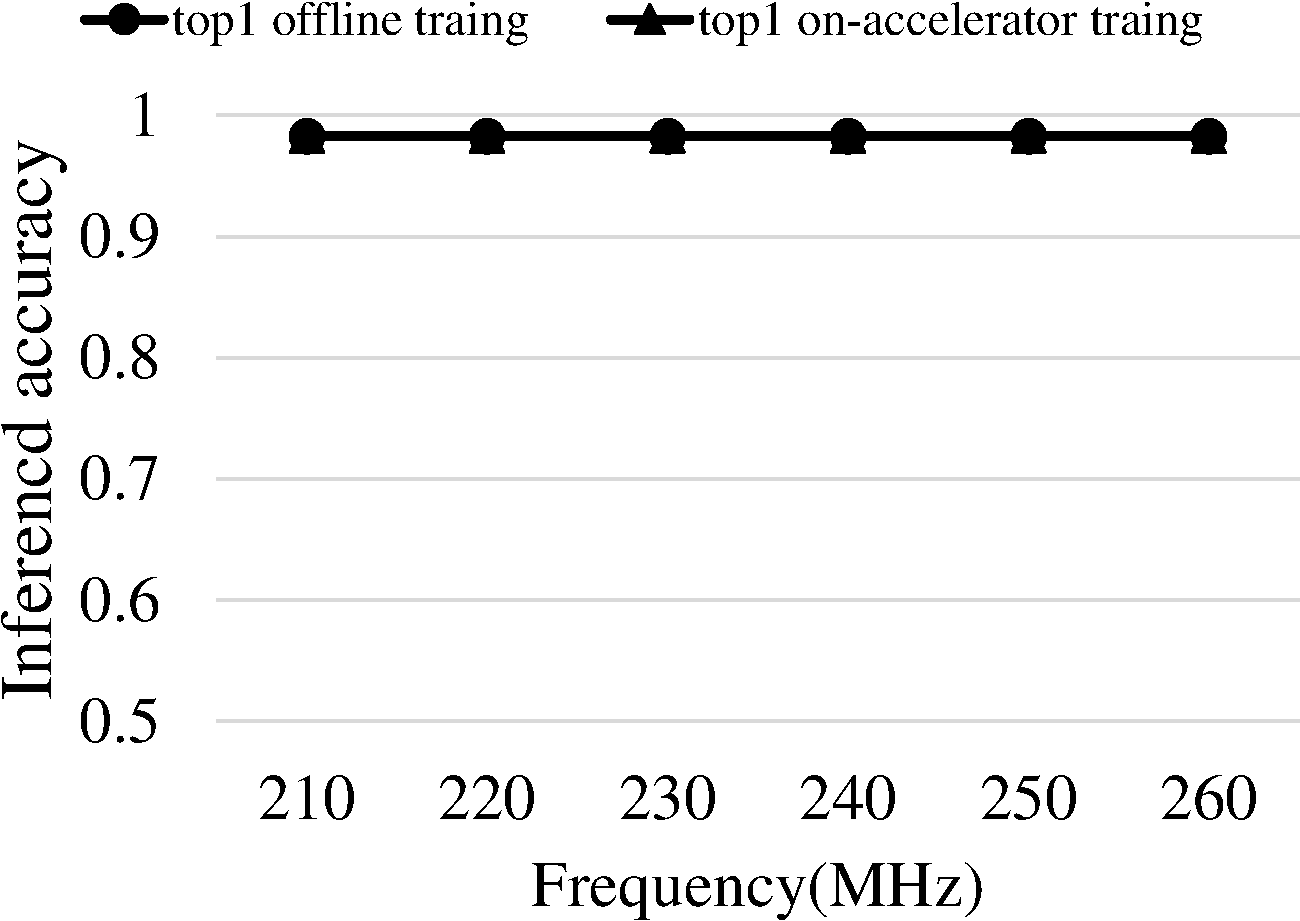
\includegraphics[width=0.6\linewidth]{lenet-overclock}
	}
	\qquad
	\subfloat[AlexNet]{
                \label{fig:alexnet}
                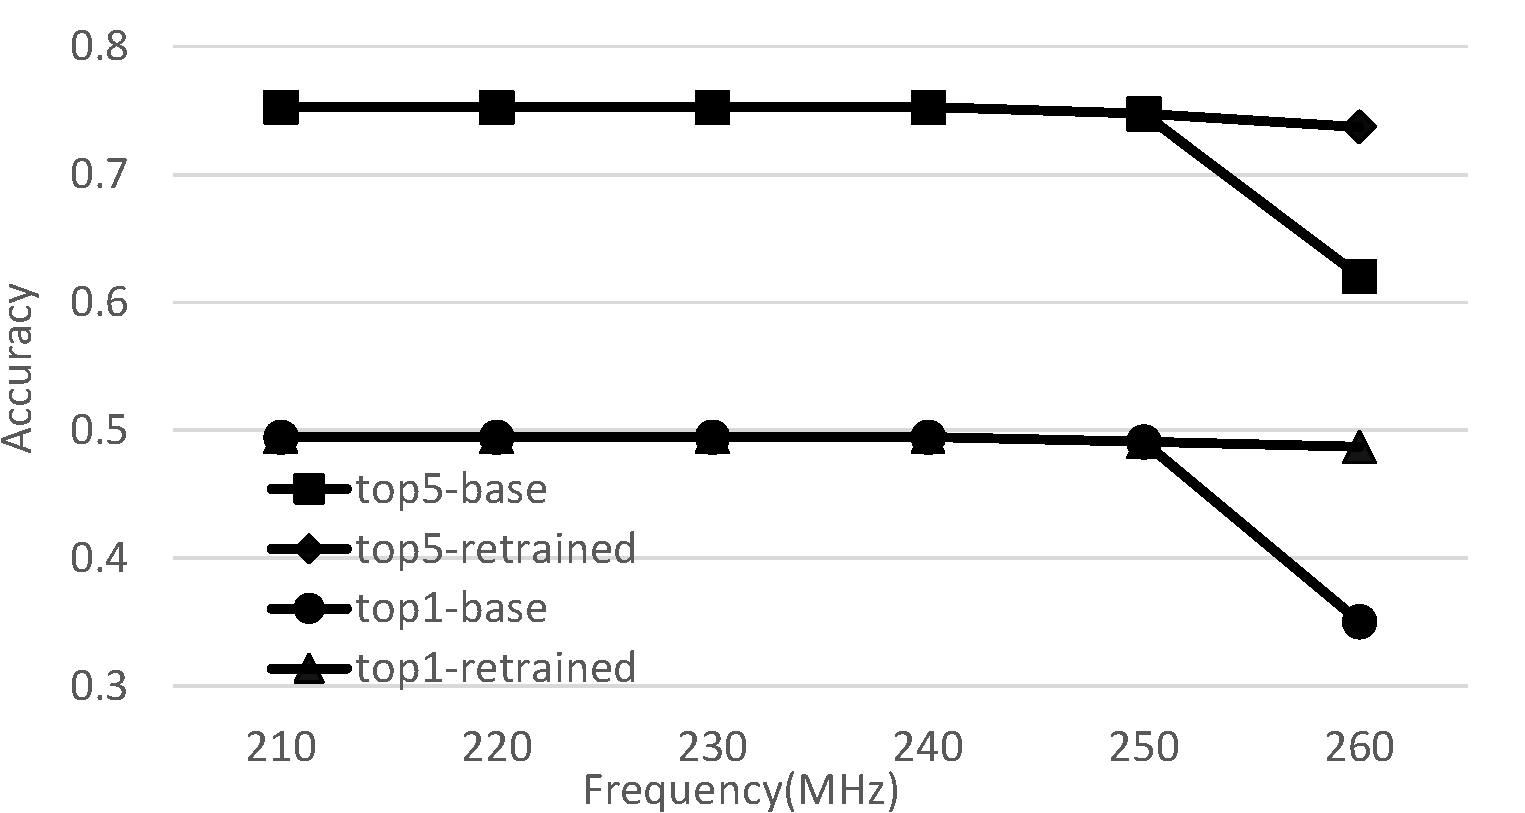
\includegraphics[width=0.6\linewidth]{alexnet-overclock}
        }
	\qquad
	\subfloat[VGG-16]{
                \label{fig:vgg16}
                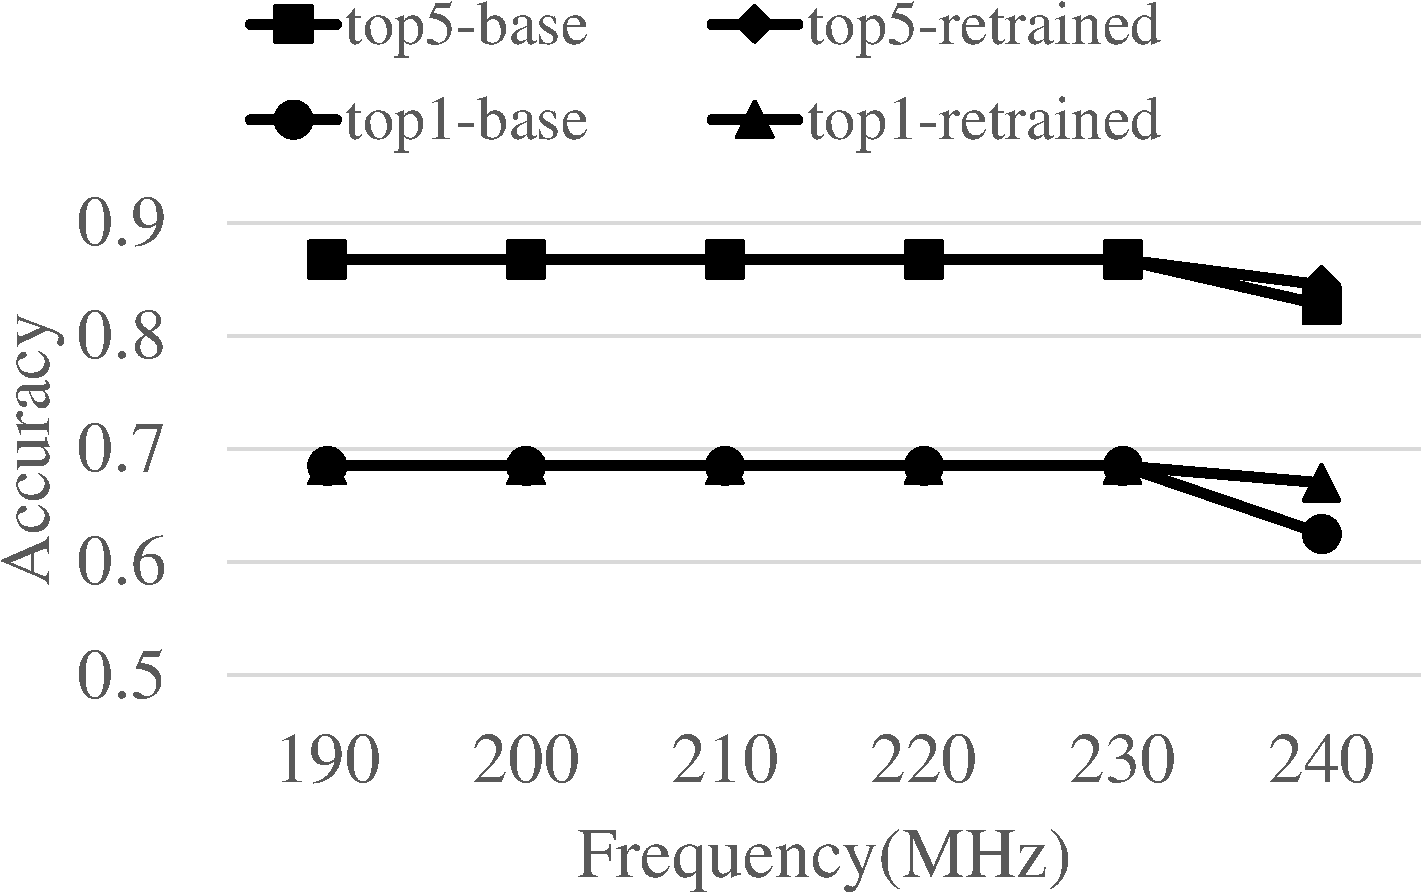
\includegraphics[width=0.6\linewidth]{vgg16-overclock}
        }
        \qquad
	\subfloat[VGG-19]{
                \label{fig:vgg19}
                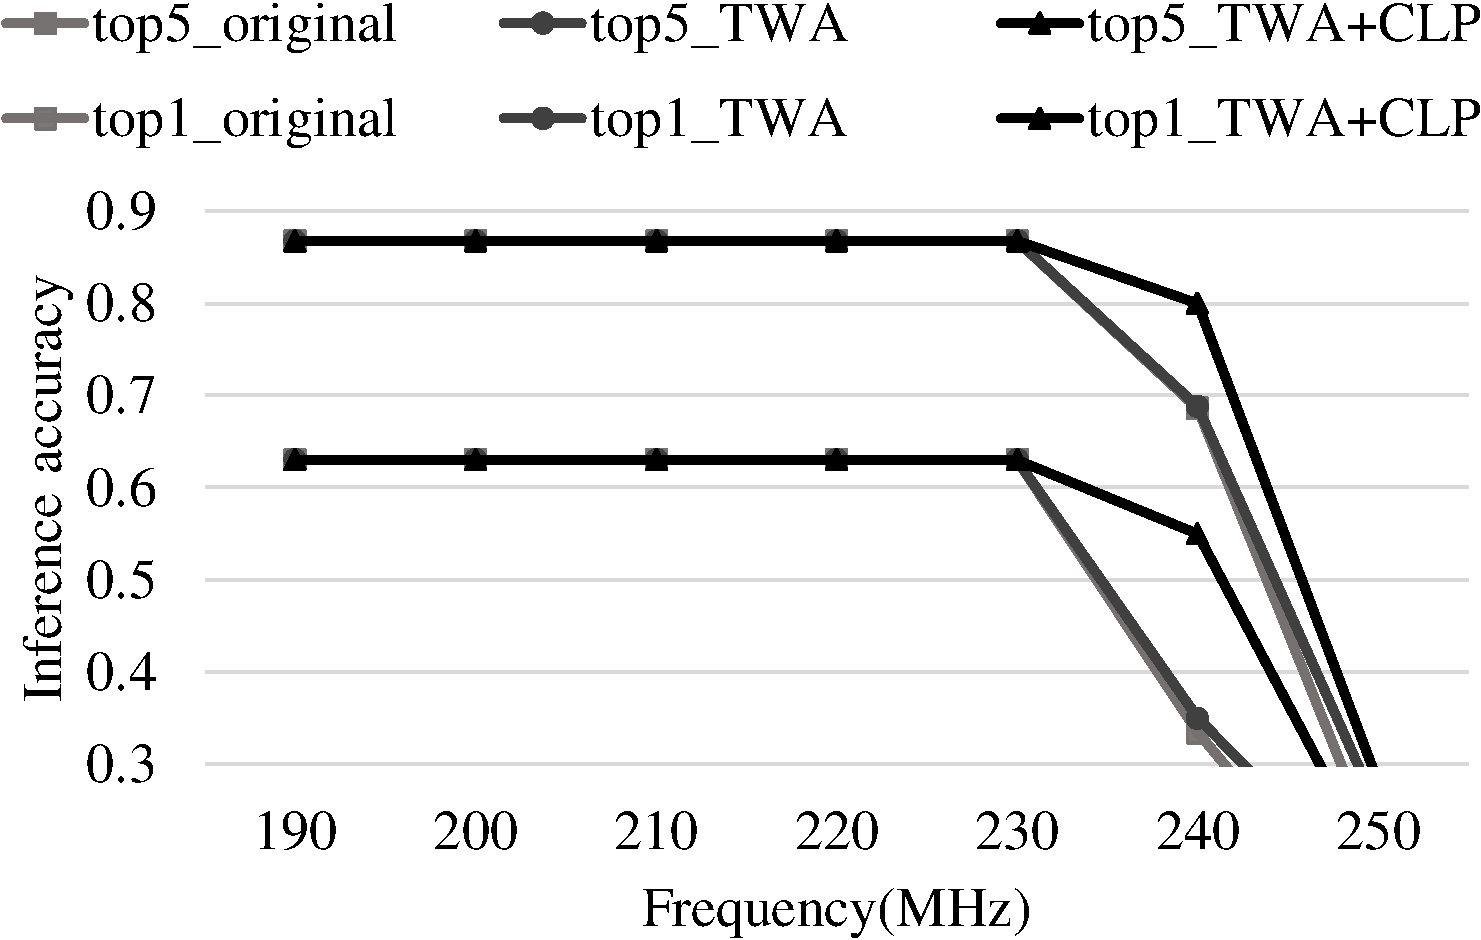
\includegraphics[width=0.6\linewidth]{vgg19-overclock}
        }
	\caption{The Accuracy of Four CNN models on accelerators with different overclocking frequency}
        \label{fig:overclock accuracy}
\end{figure}

To ensure the stability of the overclocking experiment, we 
also keep measuring the accuracy of the accelerators with extreme 
overclocking. With repeatedly running the test for up to 40 hours, 
the measured accuracy varies slightly as present in Figure 7. 
Despite the fact that the errors caused by the overclocking can be 
hardly modeled precisely at runtime, the inherent error patterns may 
still partly be captured by the CNN model with the proposed training. 
This explains the higher prediction accuracy with the retrained model. 
According to the above experiments, we can conclude that the proposed 
accelerator aware training can produce more resilient CNN model tolerating 
errors caused by intensive overclocking. 

\begin{figure}
        \center{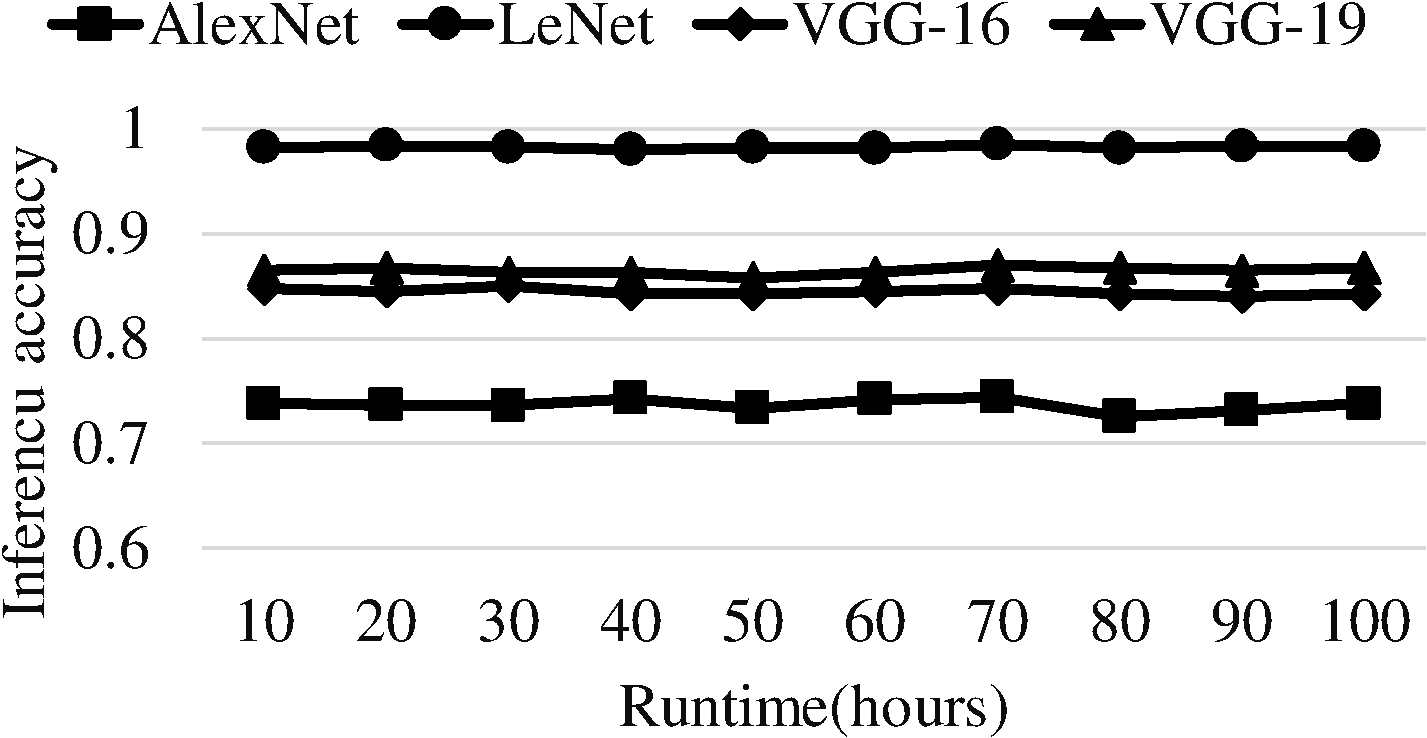
\includegraphics[width=0.6\linewidth]{stability}}
        \caption{The Stability of Retrained Model}
        \label{fig:stability}
%        \vspace{-0.5em}
\end{figure}

  Finally, we also present the training time on the hybrid CPUFPGA architecture. 
It can be seen that the training is much slower than the fixed-point training on CPU. 
This is mainly caused by the frequently data transferring between device memory and host 
memory in the proposed training, while this will not affect the inference time. In addition, 
we can also find that the training on larger network takes longer time and higher clock frequency 
is also beneficial to the training time as expected. 

\begin{figure}
        \center{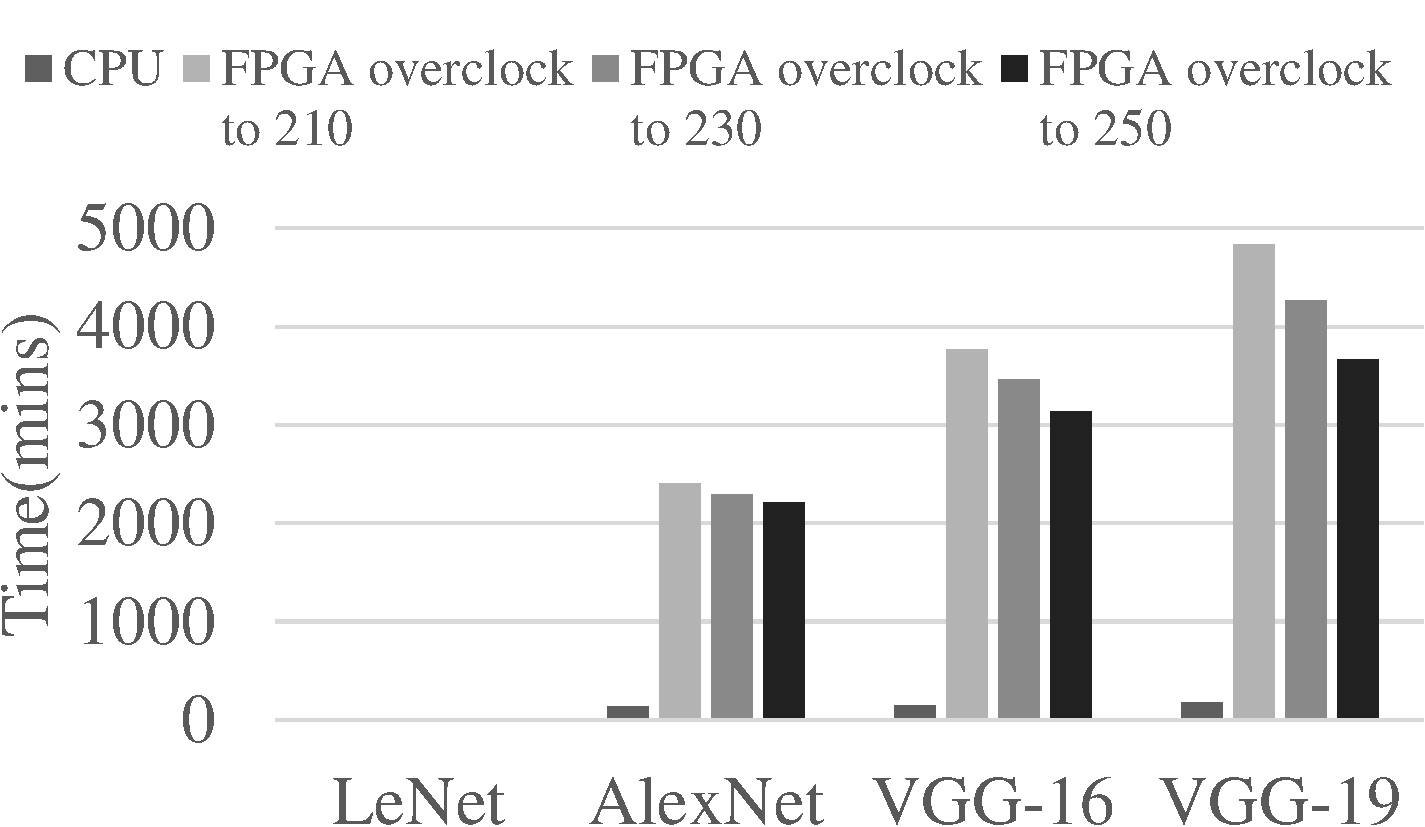
\includegraphics[width=0.6\linewidth]{time}}
        \caption{Training time}
        \label{fig:time}
%        \vspace{-0.5em}
\end{figure}

\subsection{CNN accelerator with soft errors}
  With the shrinking semiconductor feature size and increasing FPGA capacity, 
FPGA design gets error-prone to the transient faults (often known as soft errors). 
They can affect the behaviors of the FPGA design dramatically. Many researchers \cite{Mansour_20,Karim_21,Nidhin_22,Subasi_23,ROSCH_24} 
have proposed diverse approaches to address this problem. While CNN accelerators on FPGA can be different 
from general hardware design because the CNN model deployed can be further trained and tolerate the 
soft errors as proposed in prior section\cite{Tu2018RANA_1}.

  To explore the influence of soft errors on CNN accelerator, we need to inject soft errors to the system first. 
A number of fault injection techniques have been proposed in prior literature. In this work, we adopt 
a simple software simulation- based method to inject random errors. Although the error may be caused by 
on-chip memory or other SRAM cells, we have a random bit of the computing result flipped at a specific rate. 
The simple yet representative model will not increase the training time too much.

  We also take LeNet, AlexNet, VGG-16, and VGG-19 to evaluate the influence of soft errors on prediction accuracy,
the top-5 accuracy of the resulting implementations is presented in Figure 9. When we gradually 
increase the error rate from 1E-7 to 1E-5, the prediction accuracy degrades accordingly when applying the off-line 
trained model directly on the faulty accelerator. When the error rate goes up to 1E-4.5, 
the accuracy in the worst case drops by around 13.5\%. Similar to overclocking, LeNet can tolerate 
more errors than the other three networks. The accuracy remains unchanged until the error rate reaches 1E-3. 
When the error injection rate is low, the CNN model is able to cover almost all the negative influence 
on the prediction accuracy.

\begin{figure}
        \center
        \subfloat[LeNet]{
                \label{fig:lenet}
                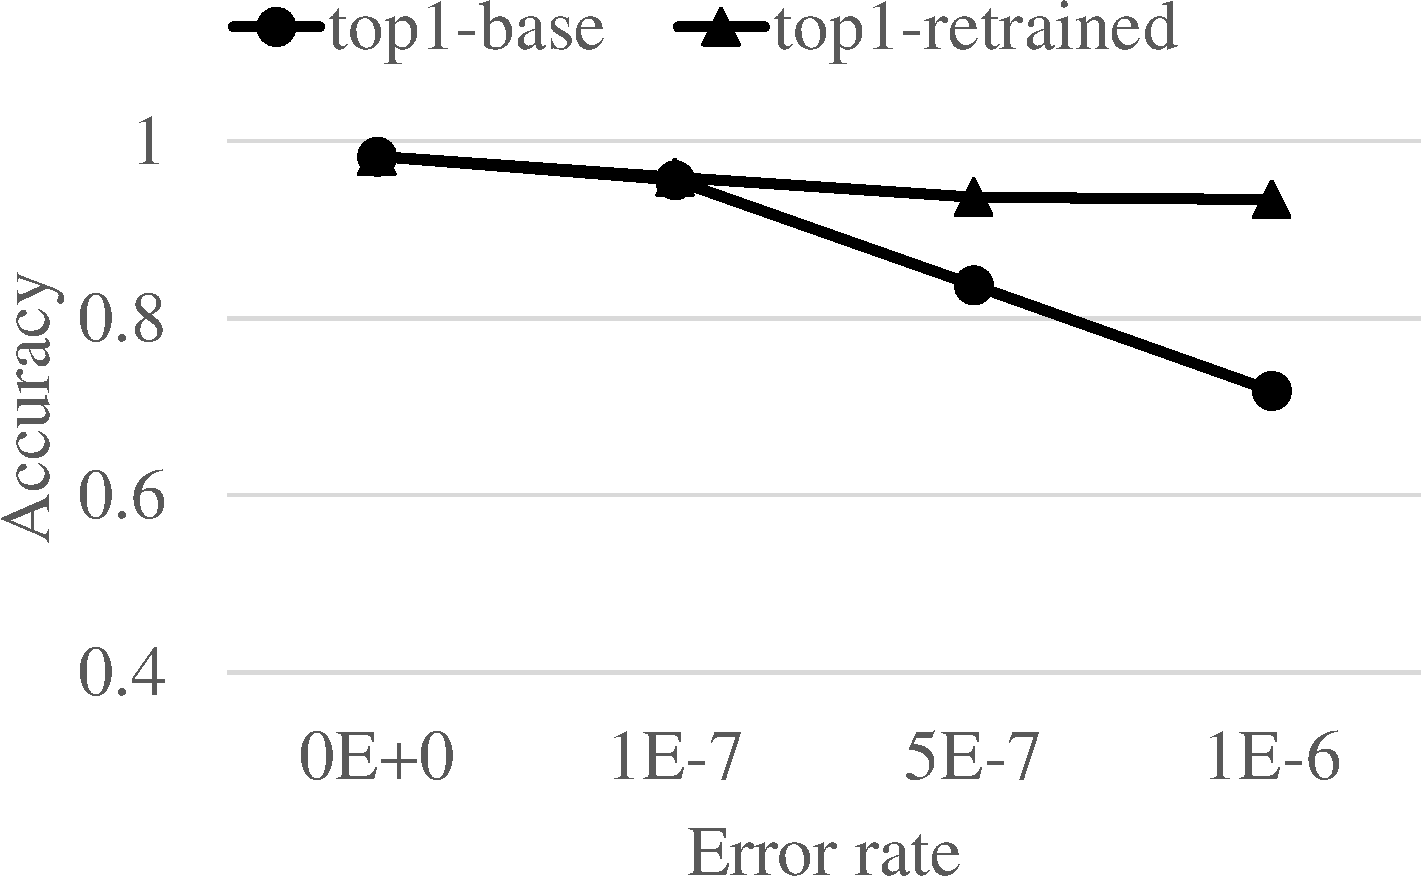
\includegraphics[width=0.6\linewidth]{lenet-softerror}
        }
        \qquad
        \subfloat[AlexNet]{
                \label{fig:alexnet}
                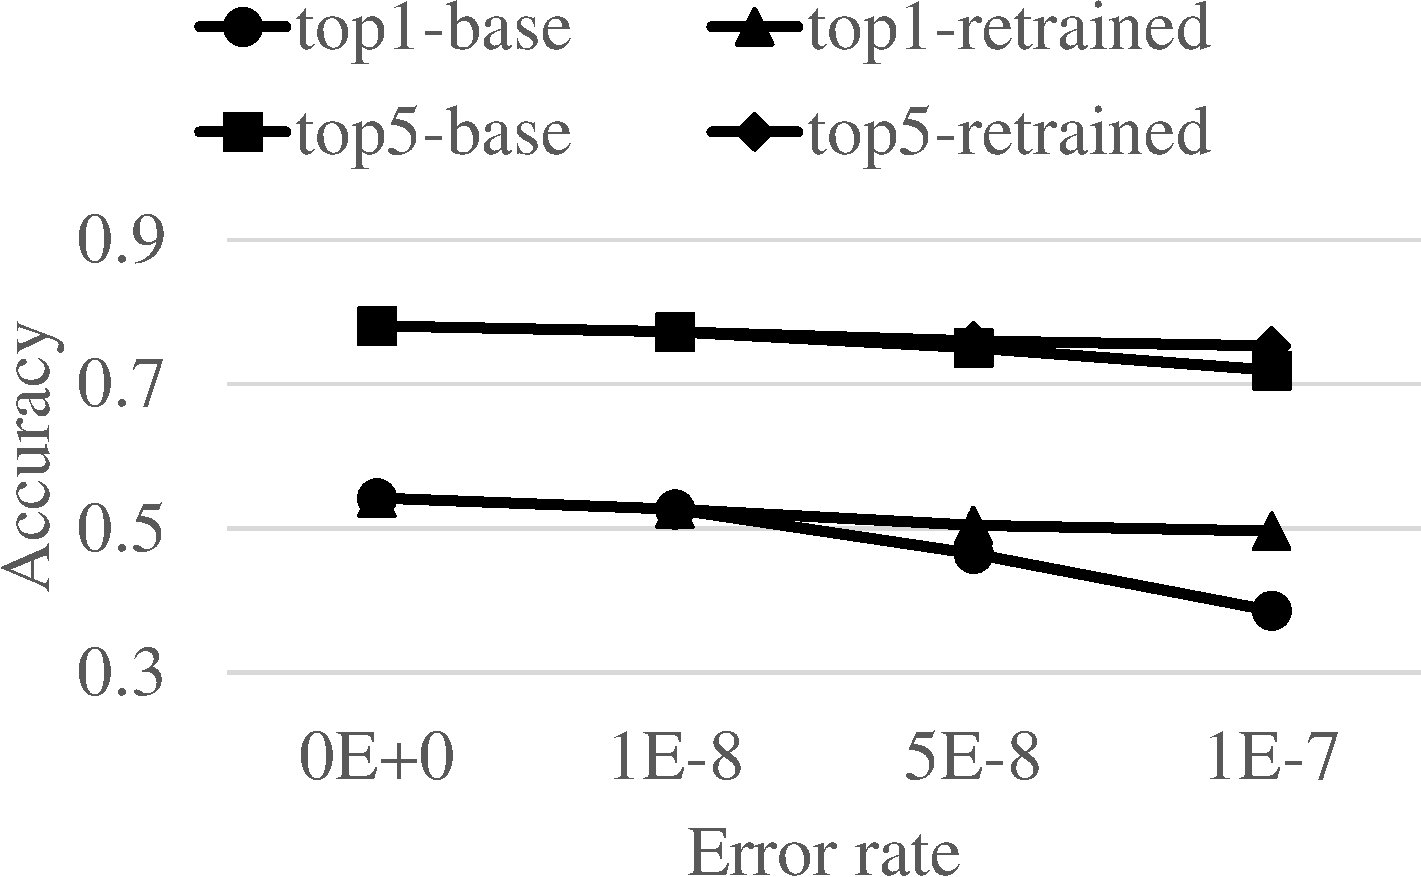
\includegraphics[width=0.6\linewidth]{alexnet-softerror}
        }
        \qquad
        \subfloat[VGG-16]{
                \label{fig:vgg16}
                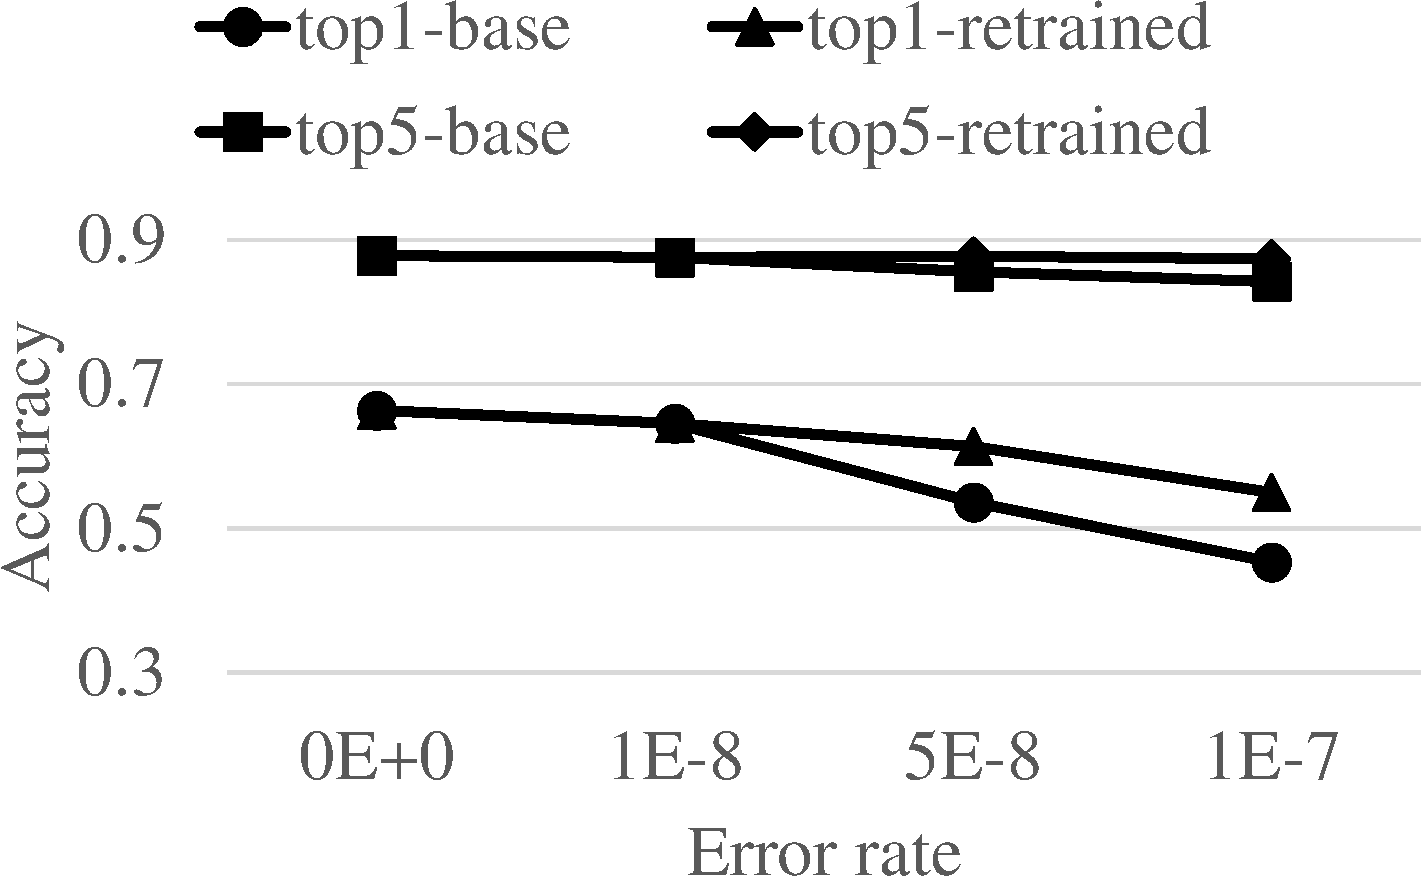
\includegraphics[width=0.6\linewidth]{vgg16-softerror}
        }
        \qquad
        \subfloat[VGG-19]{
                \label{fig:vgg19}
                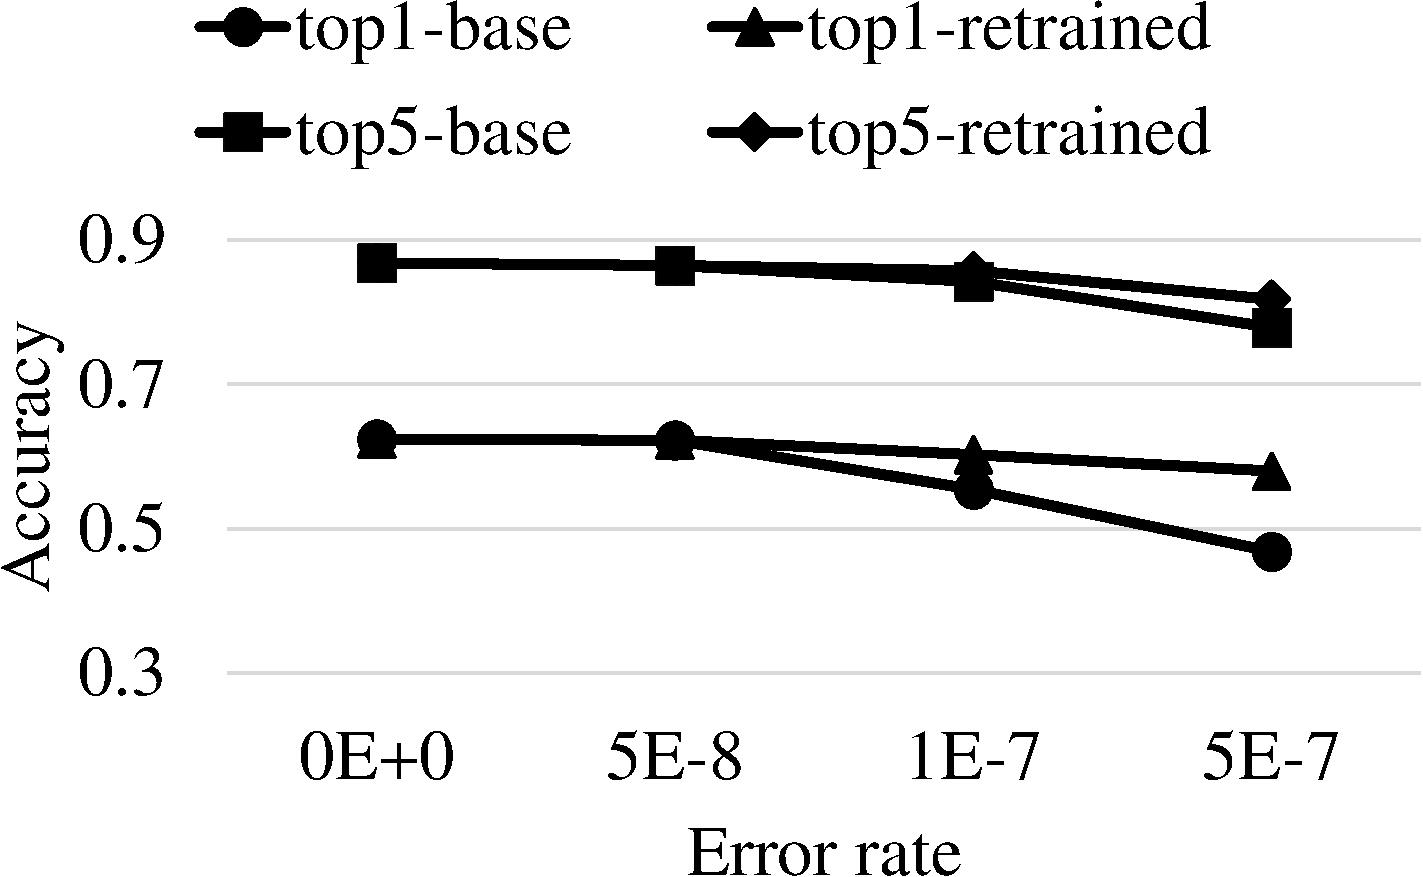
\includegraphics[width=0.6\linewidth]{vgg19-softerror}
        }
        \caption{The Precision of Four CNN models on accelerators with different error rate}
        \label{fig:softerror accuracy}
\end{figure}

  When the error injection rate goes higher, the proposed retraining becomes critical. 
According to the experiments, the accuracy of the four retrained models improve by 6.8\%, 1.5\%, 3\%, and 3\% 
respectively compared to that of the base model when the accelerators are exposed to the highest 
error injection. In summary, the experiments demonstrate that we can have the CNN model to learn 
both the characteristics of the data and the underlying ‘undeterministic’ behaviors of the accelerator 
together using the proposed training framework. The resulting CNN model can improve the accuracy 
without any modification on the accelerator when there is high error injection rate.  


